\section{Muon ghosts}
\subsection{The DT System}
\label{DTSystem}
The drifttube (DT) system of the muon detector at CMS consists of several organization structures.\\
The smallest structure, the drift tubes are organized within a superlayer (SL). A superlayer consists of four layers of DTs. Every sector per wheel in CMS has four muon stations, counted 1 to 4 beginning with the inner most station.\\
A muon station is the composition of two SLs oriented in $\phi$ direction (stations 1-4) and one SL in $\theta$ direction (stations 1-3). The readout hardware of one station is assembled in a minicrate (MC).\\
The trigger chain of the DT system starts within a SL. Nine of the DTs are combined to a bunch and track identifier (BTI) Trigger. BTI Triggers have an overlap region to avoid inefficiencies and to obtain redundancy. If three of four DTs see a signal for a certain bunch crossing, a low quality trigger (LTRG) is generated. If four DTs in line see a signal, a high quality trigger (HTRG) is generated. For now, only HTRG are processed in the next trigger step.\\
The track correlator (TRACO) combines the HTRG of the two BTIs of the SL in phi direction within one station. TRACO triggers can be generated for muons with an angle of $45^{\circ}$ \cite{bunchedBeamTest} or less.\\
These TRACO triggers are transmitted via 40 line flat cables to the trigger server (TS). The TS is located on the MC of station 4.\\
The TS consists of a phi and a theta part. The TS phi correlates the TRACO tracks in phi direction. The TS theta correlates the tracks in $\theta$.\\
This data is transmitted via low voltage differential signaling (LVDS) to the sector collector (SC) that is located in the service cavern (USC).\\
From there the signal is processed to the global muon trigger (GMT) and the global trigger (GT).
For the setup of the muon trigger system, see also \cite{cmsMuonProject}.
\subsection{Reconstruced Ghosts}
\subsubsection{Ghost definition}
Ghosts are faked muons that are detected by the muon system although there is no physical muon present.
Muon ghosts can occur in all stages of the detection and reconstruction system of CMS beginning with the low level triggers up to the final reconstructed data (Fig. \ref{fig:ghosts}).
A ghost can also be a detected muon that has the wrong time stamp and thus is assigned to the wrong bunch crossing.

\subsubsection{Reco ghosts}
Following the definition of ghosts, a RECO ghost is a reconstructed muon that has no matching generated (GEN) muon.\\
For this matching, for every RECO muon the nearest GEN muons in terms of $\Delta R$ is determined. Additionally, the vertex position of the GEN and RECO muon must not be displaced by $>$ 0.1 cm in every of the three coordinates to assure that the RECO muon is not from a pileup event.\\
The following investigations are performed with global muons only, to have both the muon system and tracker information available for every muon. Furthermore, the eta direction of the investigated muons is cut to be abs(eta) $<$ 0.8 to check for muons in the barrel region only. The sample used is a ZZ$\to$4l with 2012 conditions.\\
$\Delta R$ is plotted (Fig. \ref{DeltaRDistribution}) for all GEN muons with their matched RECO muon. If two RECO muons match the same GEN muon, $\Delta R$ is plotted for both RECO muons.\\
Most of the matched muons have a very small $\Delta R$. Only a few muons have a $\Delta R$ above 0.1 with a maximum at 1.5. It is obvious that the most muon combinations with $\Delta R > 0.1$ come from muons in ghost events. Therefore, a separation between ghosts and real muons using $\Delta R$ seems to be feasible and is discussed.
\begin{figure}[b]
\centering
\begin{minipage}[t]{0.95\textwidth}
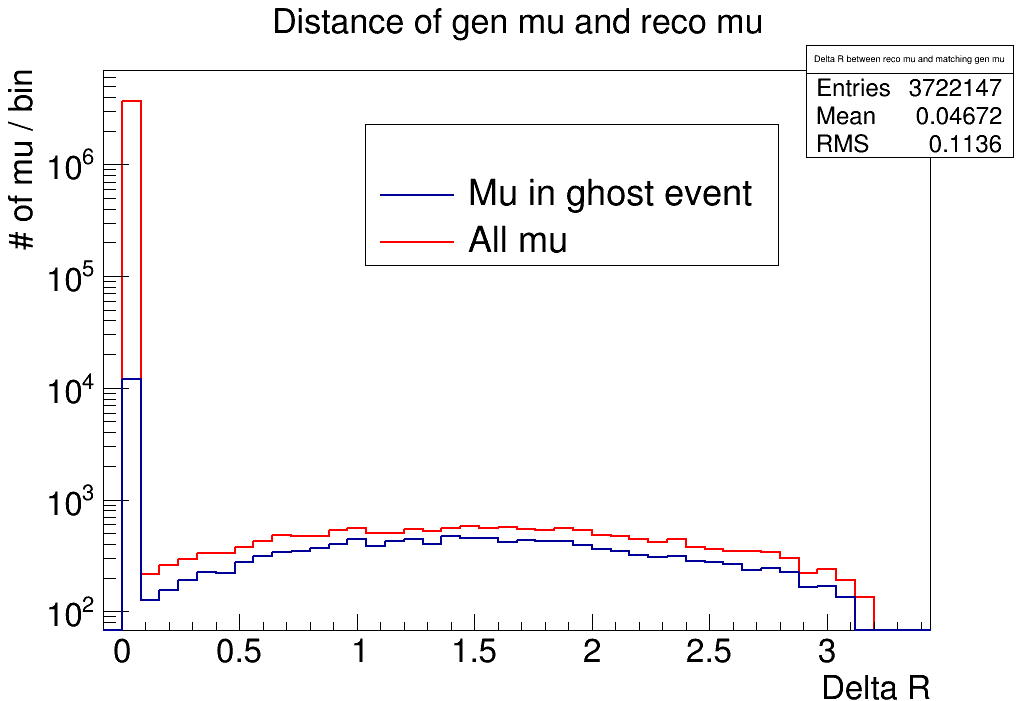
\includegraphics[width=\textwidth]{Figures/scheuch/Trennung.png}
\caption{$\Delta R$ between all RECO muons and the matched GEN muon in all events and in events that are marked as ghost events}
\label{DeltaRDistribution}
\end{minipage}
\end{figure}
If one GEN muon has two or more associated RECO muons all but one of these RECO muons are considered to be ghosts. An event with at least one ghost is named ghost event.\\
For the separation whether a RECO muon is a ghost or real, a $\Delta R$ cut is introduced. If the $\Delta R$ between RECO muon and associated GEN muon is smaller than 0.1, the muon is considered to be a correctly reconstructed muon. If the $\Delta R$ is greater than 0.1, it is considered to be a ghost.

\subsubsection{Matching efficiency and quality of separation}
To determine whether the matching algorithm is correct and efficient, some control variables have been studied.\\
The distance of the vertex position in the z direction (along the beam axis) of the RECO muon and the associated GEN muon was plotted (see Fig. \ref{DeltaZMatching}). The distance is within the resolution of the tracker system. Nevertheless, all muons with a distance of more than 0.1 cm are rejected, since for large distances in the z vertex difference a mismatching can not be imposed.\\
\begin{figure}[b]
\centering
\begin{minipage}[t]{0.95\textwidth}
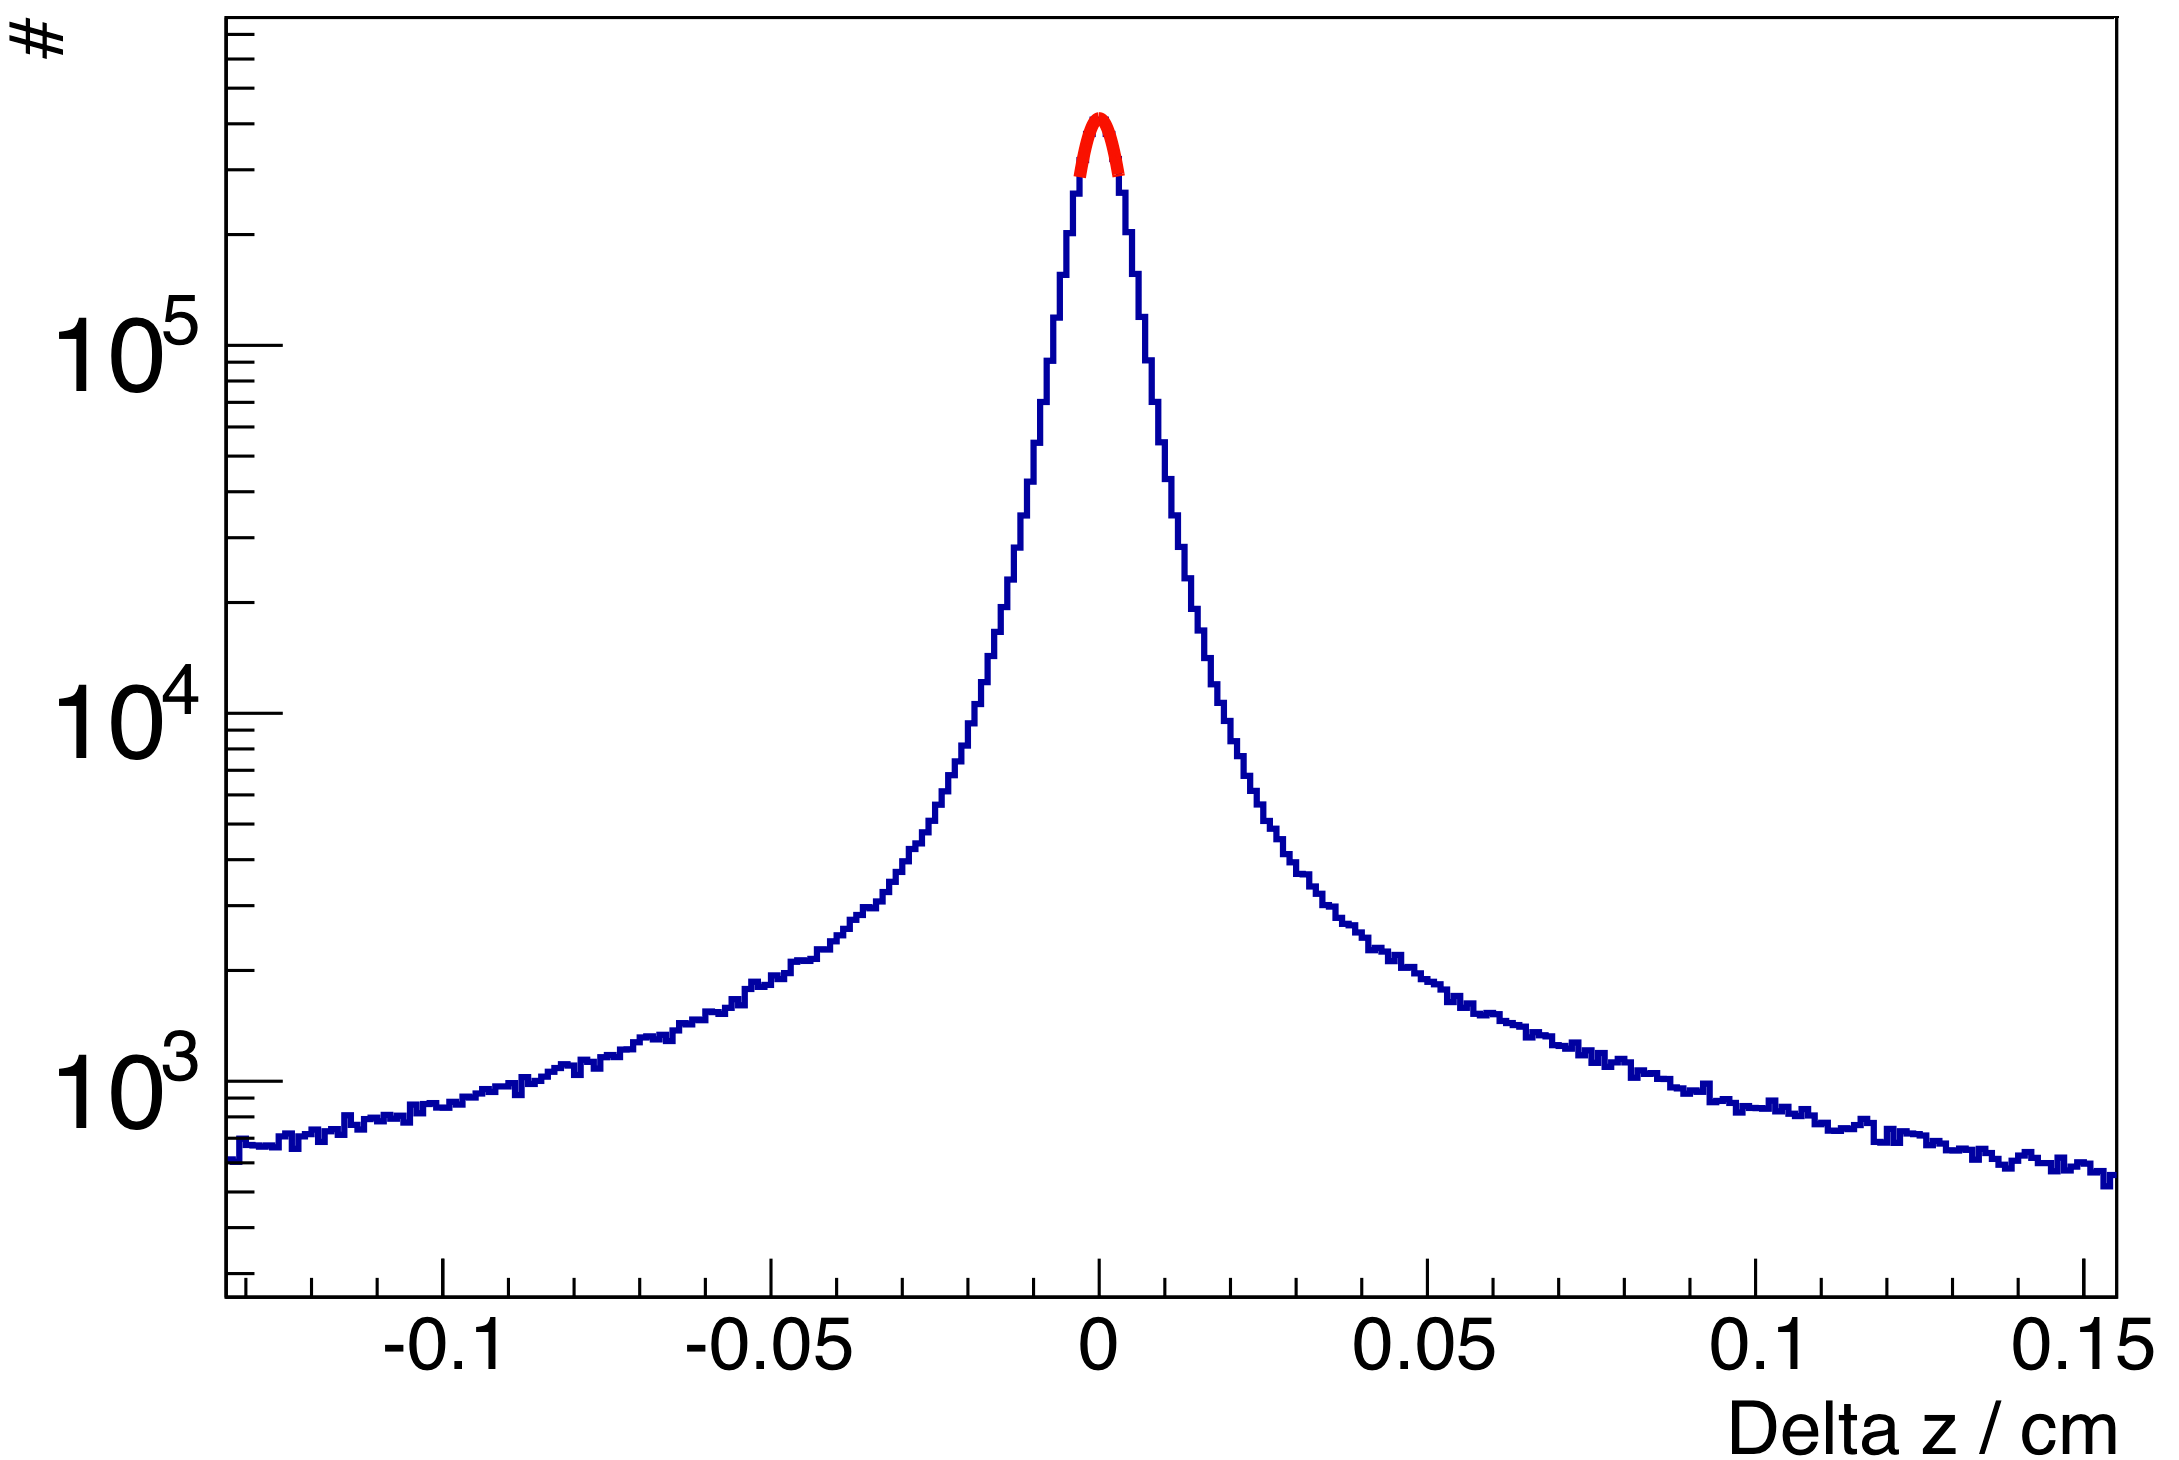
\includegraphics[width=\textwidth]{Figures/scheuch/DeltaZ.png}
\caption{Distance of the z position of the vertex RECO muon and the matched GEN muon}
\label{DeltaZMatching}
\end{minipage}
\end{figure}
To show that the determination between ghost and real muon is reliable, the $p_{T}$ ratio between GEN muon and RECO muon is plotted for identified ghosts (see Fig. \ref{PtRatioGhost}) and real muons within a ghost event (see Fig. \ref{PtRatioReal}).
\begin{figure}[b]
\centering
\begin{minipage}[t]{0.475\textwidth}
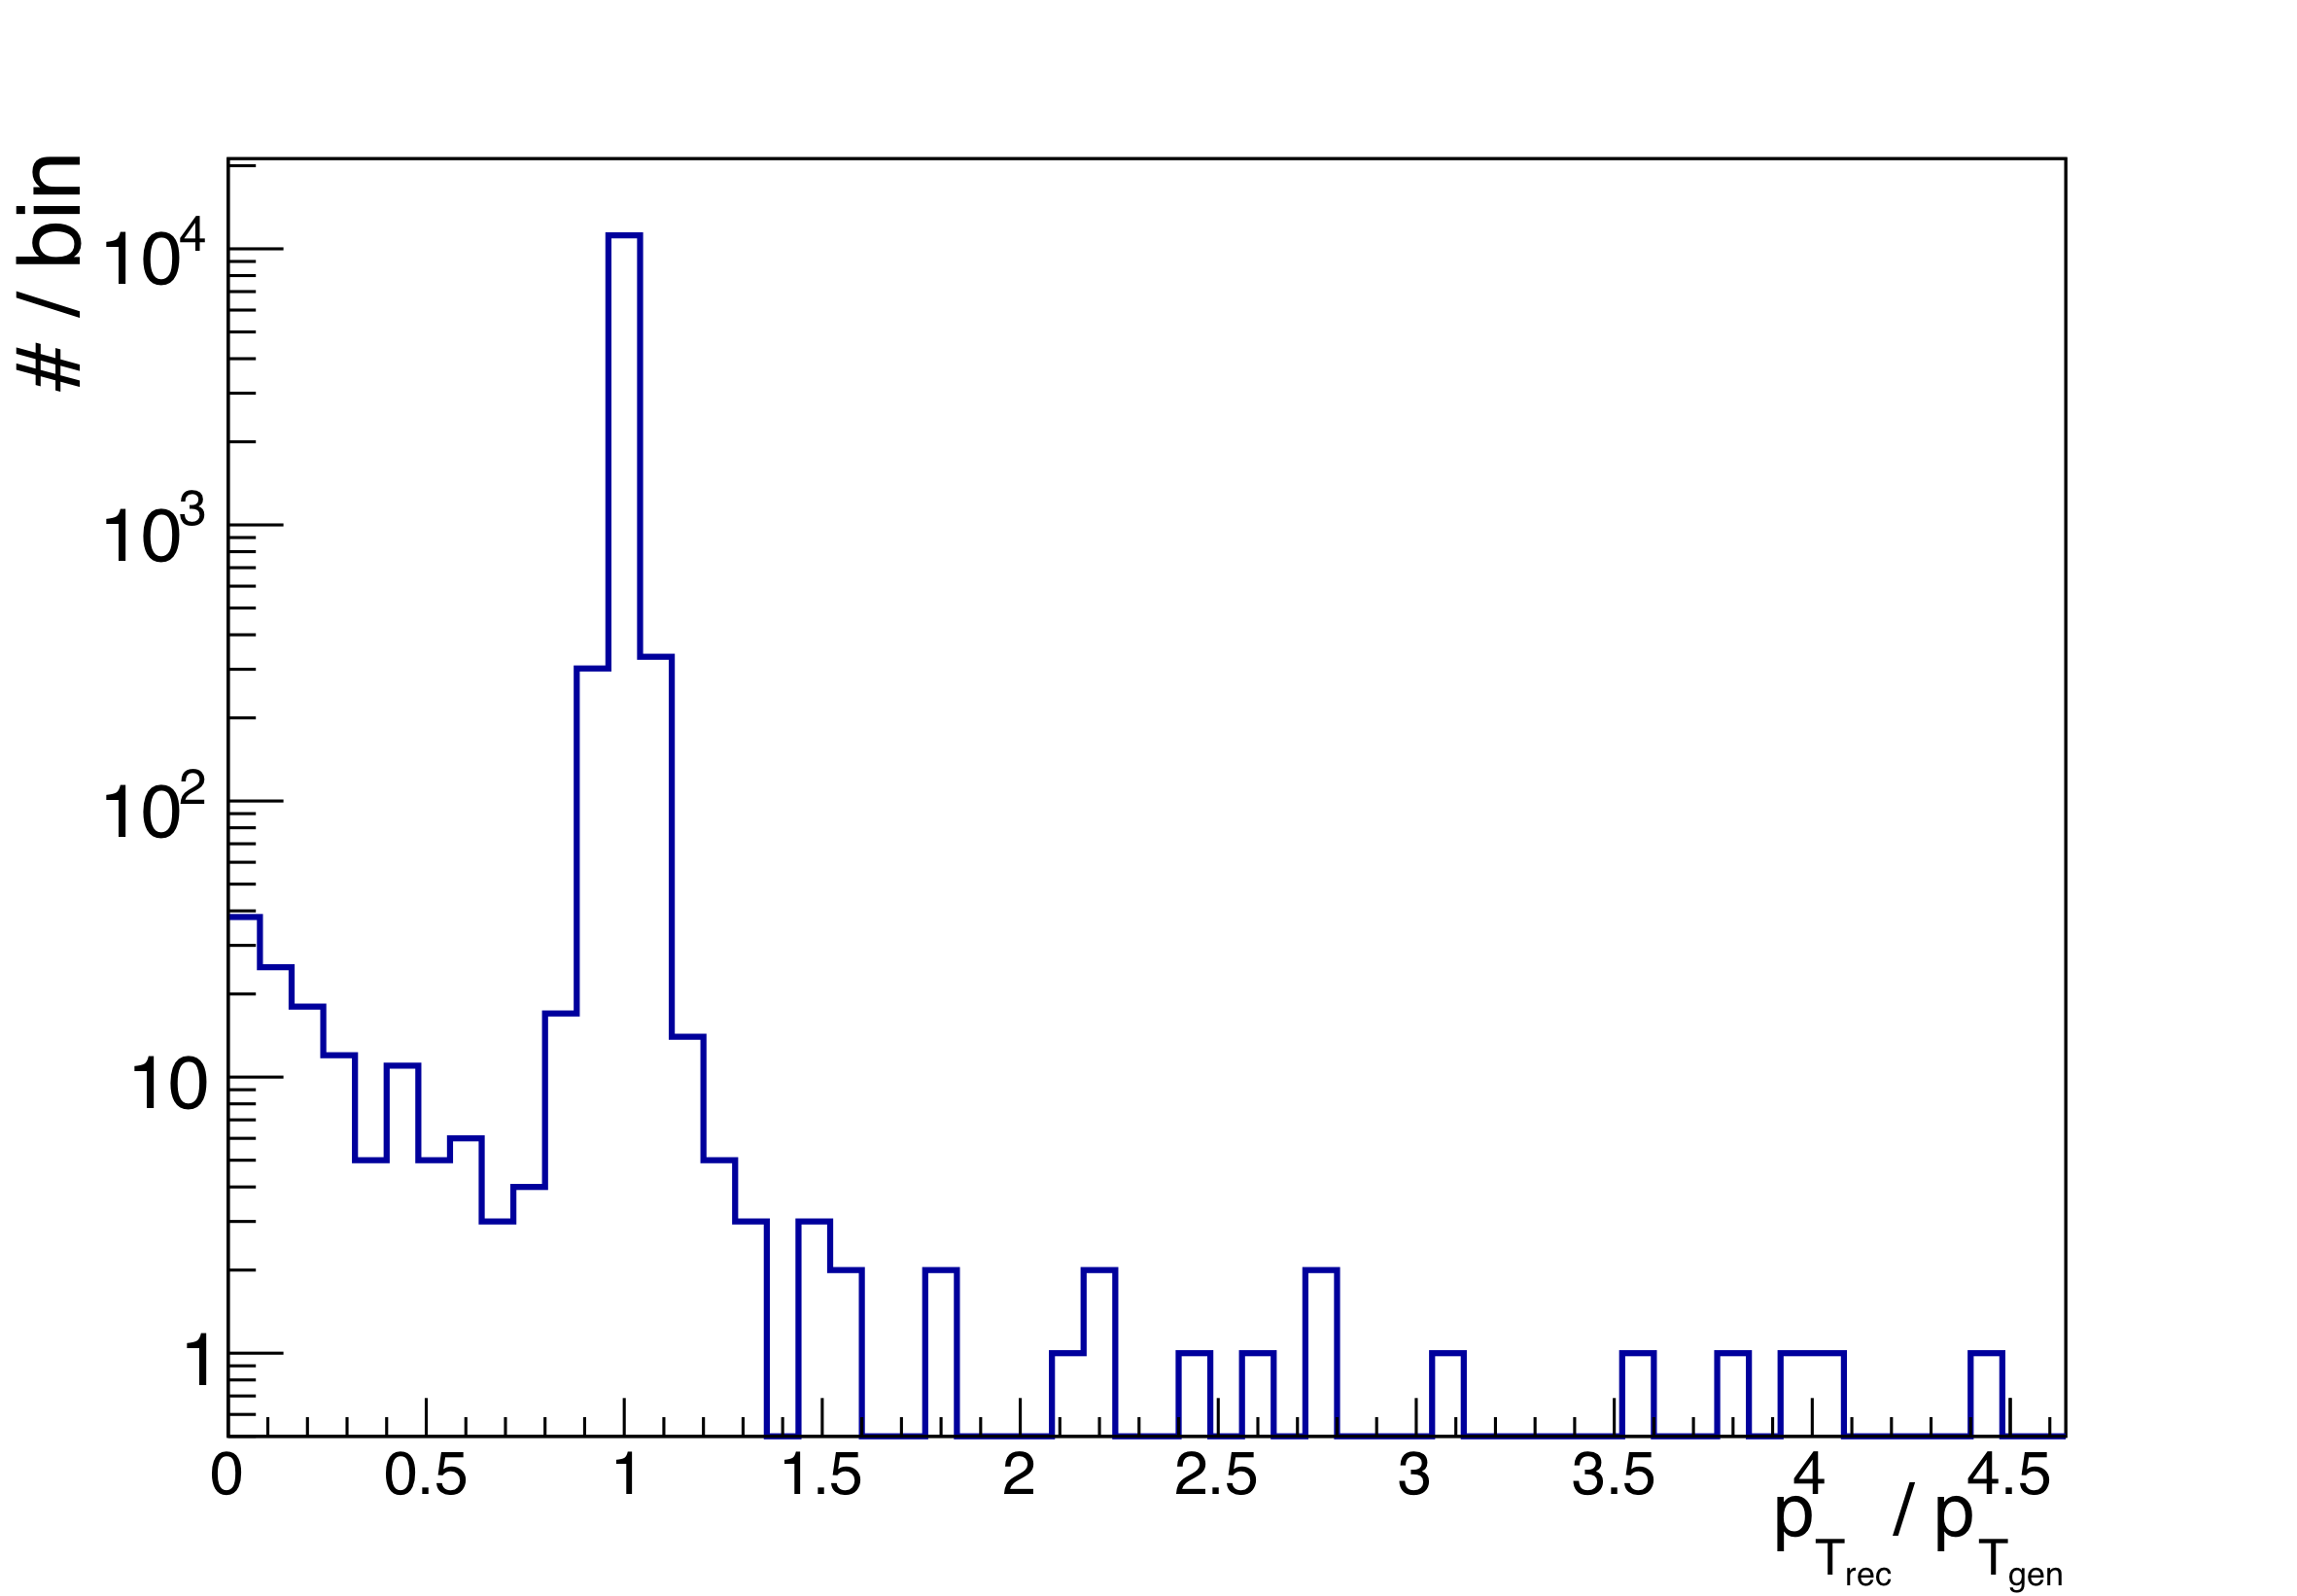
\includegraphics[width=\textwidth]{Figures/scheuch/ptRatioRealMu.png}
\caption{$\mathrm{p_{T}}$ ratio of the GEN and RECO mu for identified real RECO muons}
\label{PtRatioReal}
\end{minipage}
\hspace{0.5cm}
\begin{minipage}[t]{0.475\textwidth}
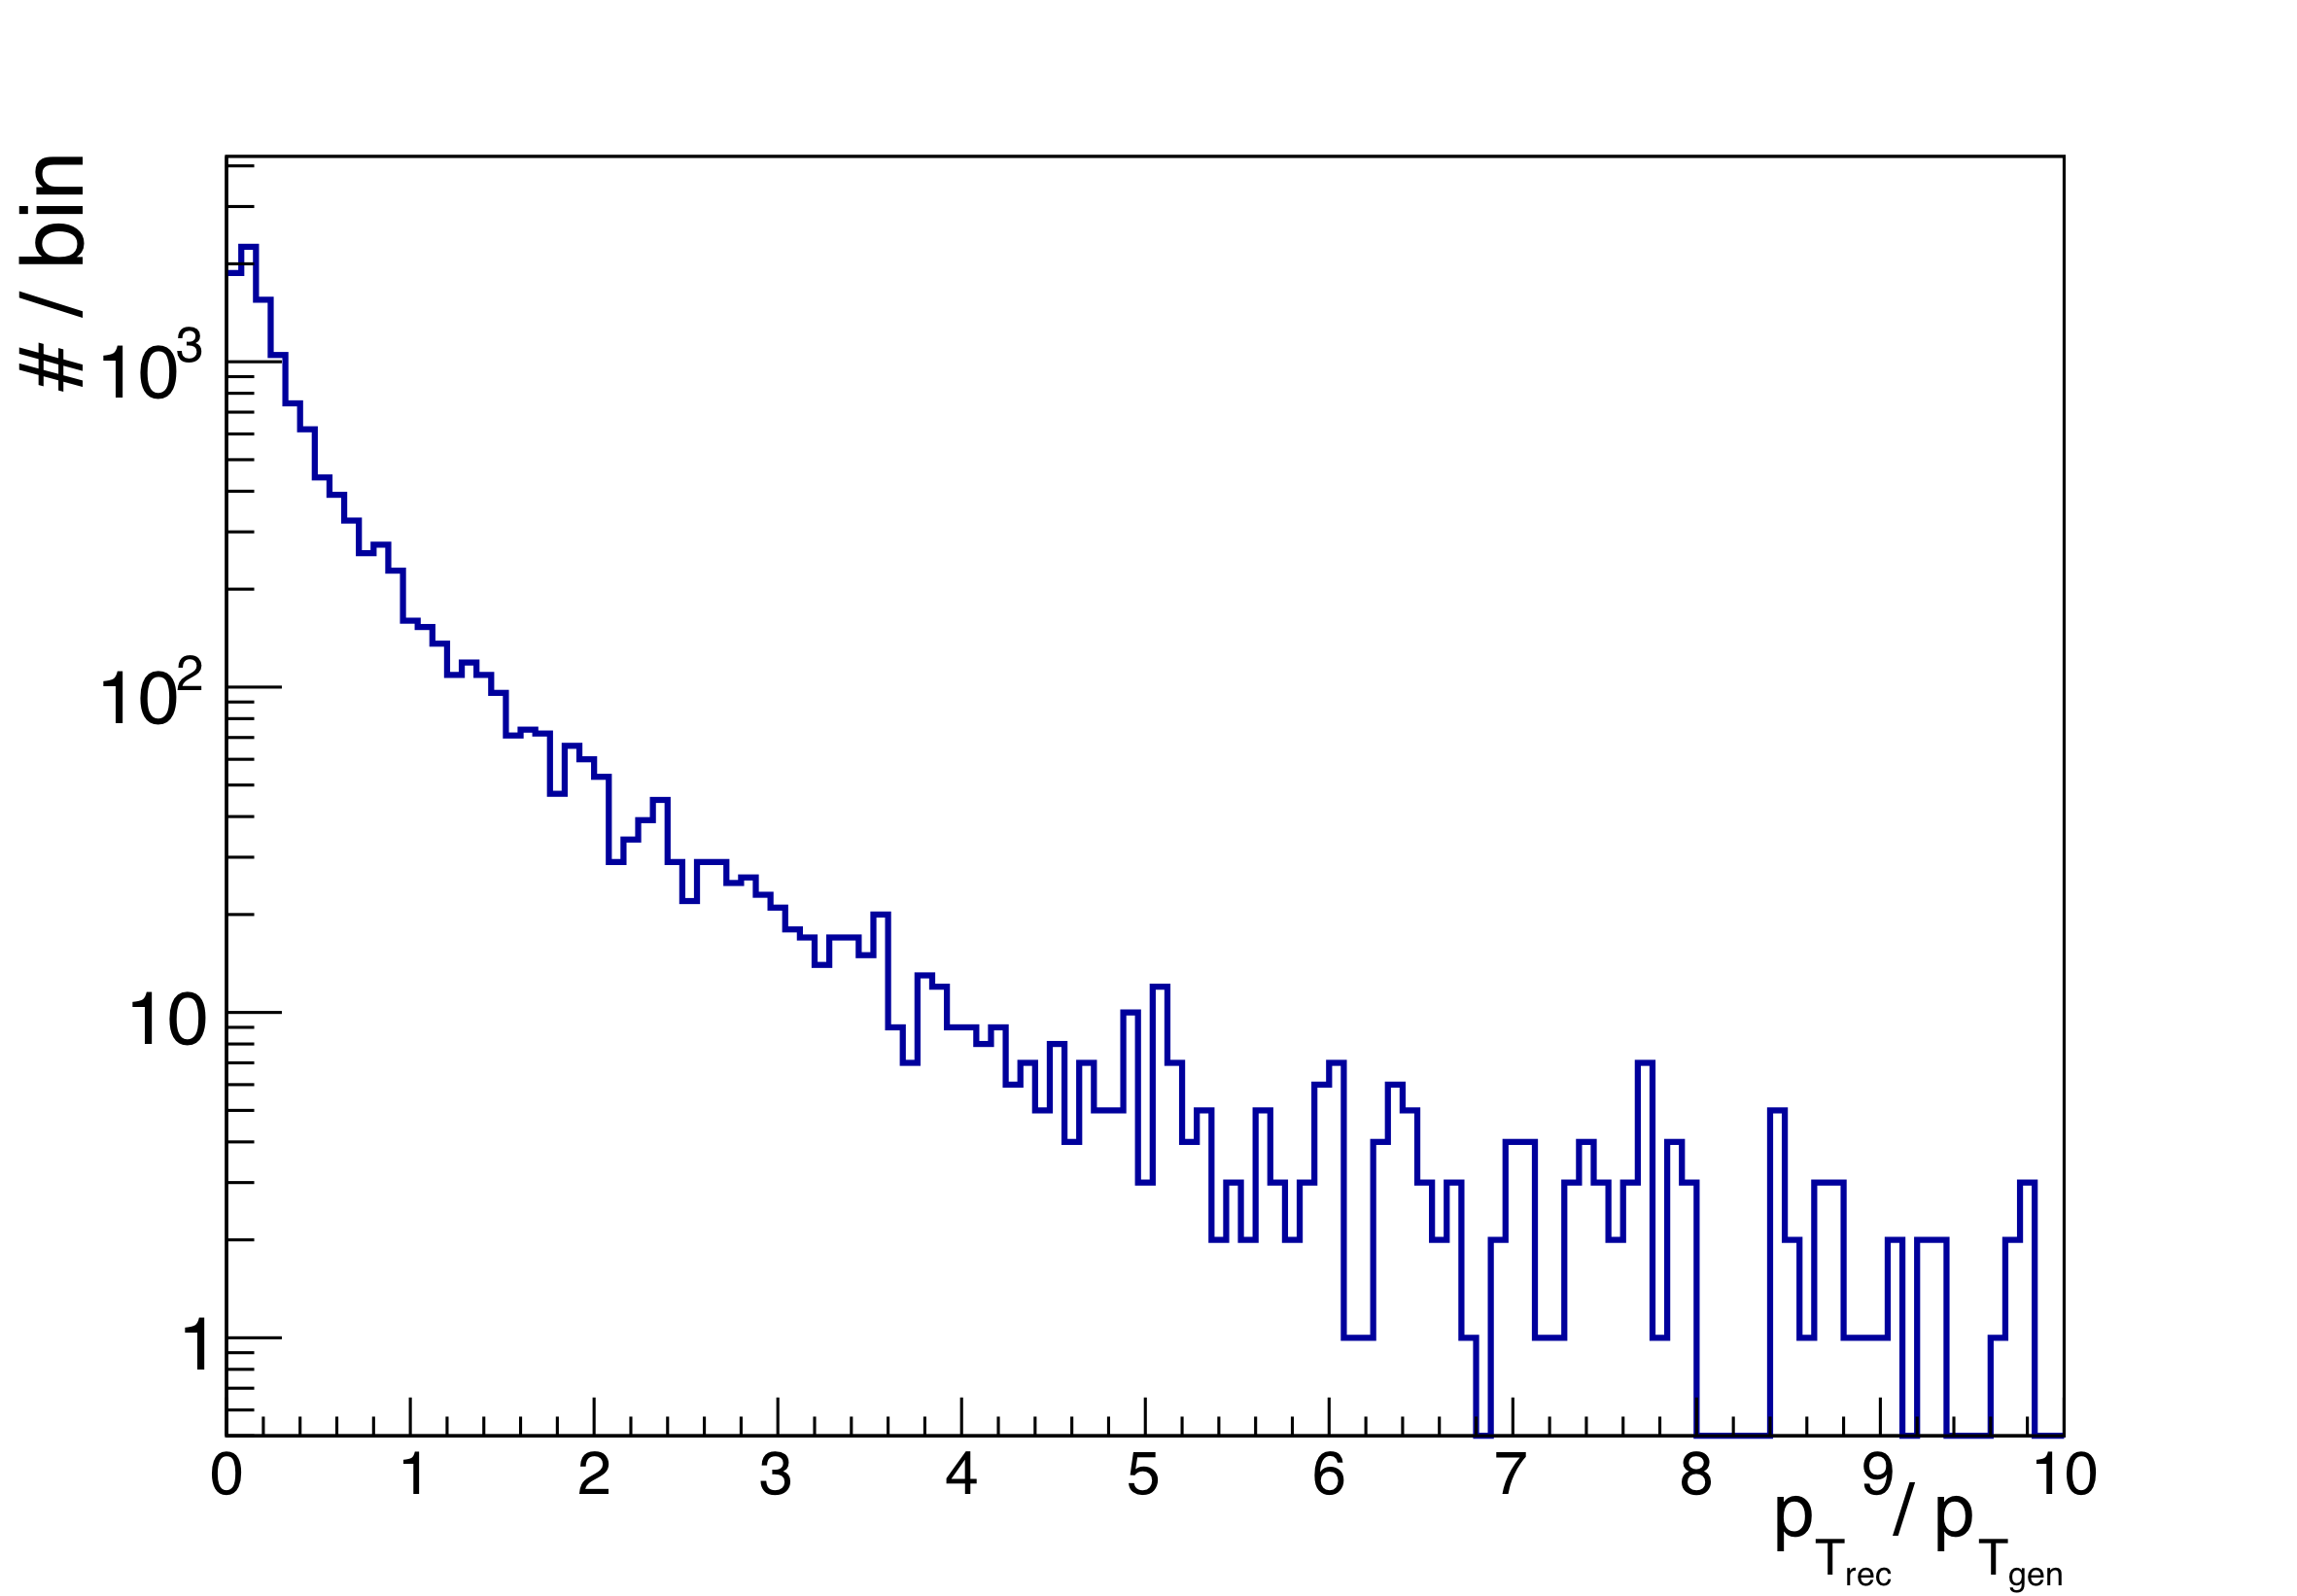
\includegraphics[width=\textwidth]{Figures/scheuch/ptRatioGhosts.png}
\caption{$\mathrm{p_{T}}$ ratio of the GEN and RECO mu for identified RECO ghosts}
\label{PtRatioGhost}
\end{minipage}
\end{figure}
The $p_{T}$ ratio peaks at 1 for real muons. This indicates that the RECO muon is in fact the correct reconstruction of the generated particle. On the other hand, the $p_{T}$ ratio of the ghost muons shows a non peaking shape. Therefore, it can be assumed that the $p_{T}$ of the ghosts is not related to the matched GEN particle. The $p_{T}$ of the ghost is smaller than the $p_{T}$ of the generating particle in the majority of ghost events.\\
Furthermore, under the assumption that there is only one ghost per real muon in the majority of the events, one expects that the number of ghosts and real muons is equal for a certain GEN muon. Comparing the number of ghosts (12175) and the number of real muons (12013) shows that the seperation between the real and the ghost muon is working well.

\subsubsection{Ghost busting with HO information}
To determine whether hadron outer (HO) information can be used to bust ghosts on L1 Level, the whole calorimeter (including HCAL and ECAL) information is used for 2012 simulations, since HO did not work properly during this phase. In a first step, the likelihood ratio of the calorimeter system (ECAL, HCAL, HO) defined as
\begin{equation}
L=\frac{L_{\mathrm{muon}}}{L_{\mathrm{muon}} + L_\mathrm{not\ muon}}
\end{equation}
is plotted.
\begin{figure}[b]
\centering
\begin{minipage}[t]{0.95\textwidth}
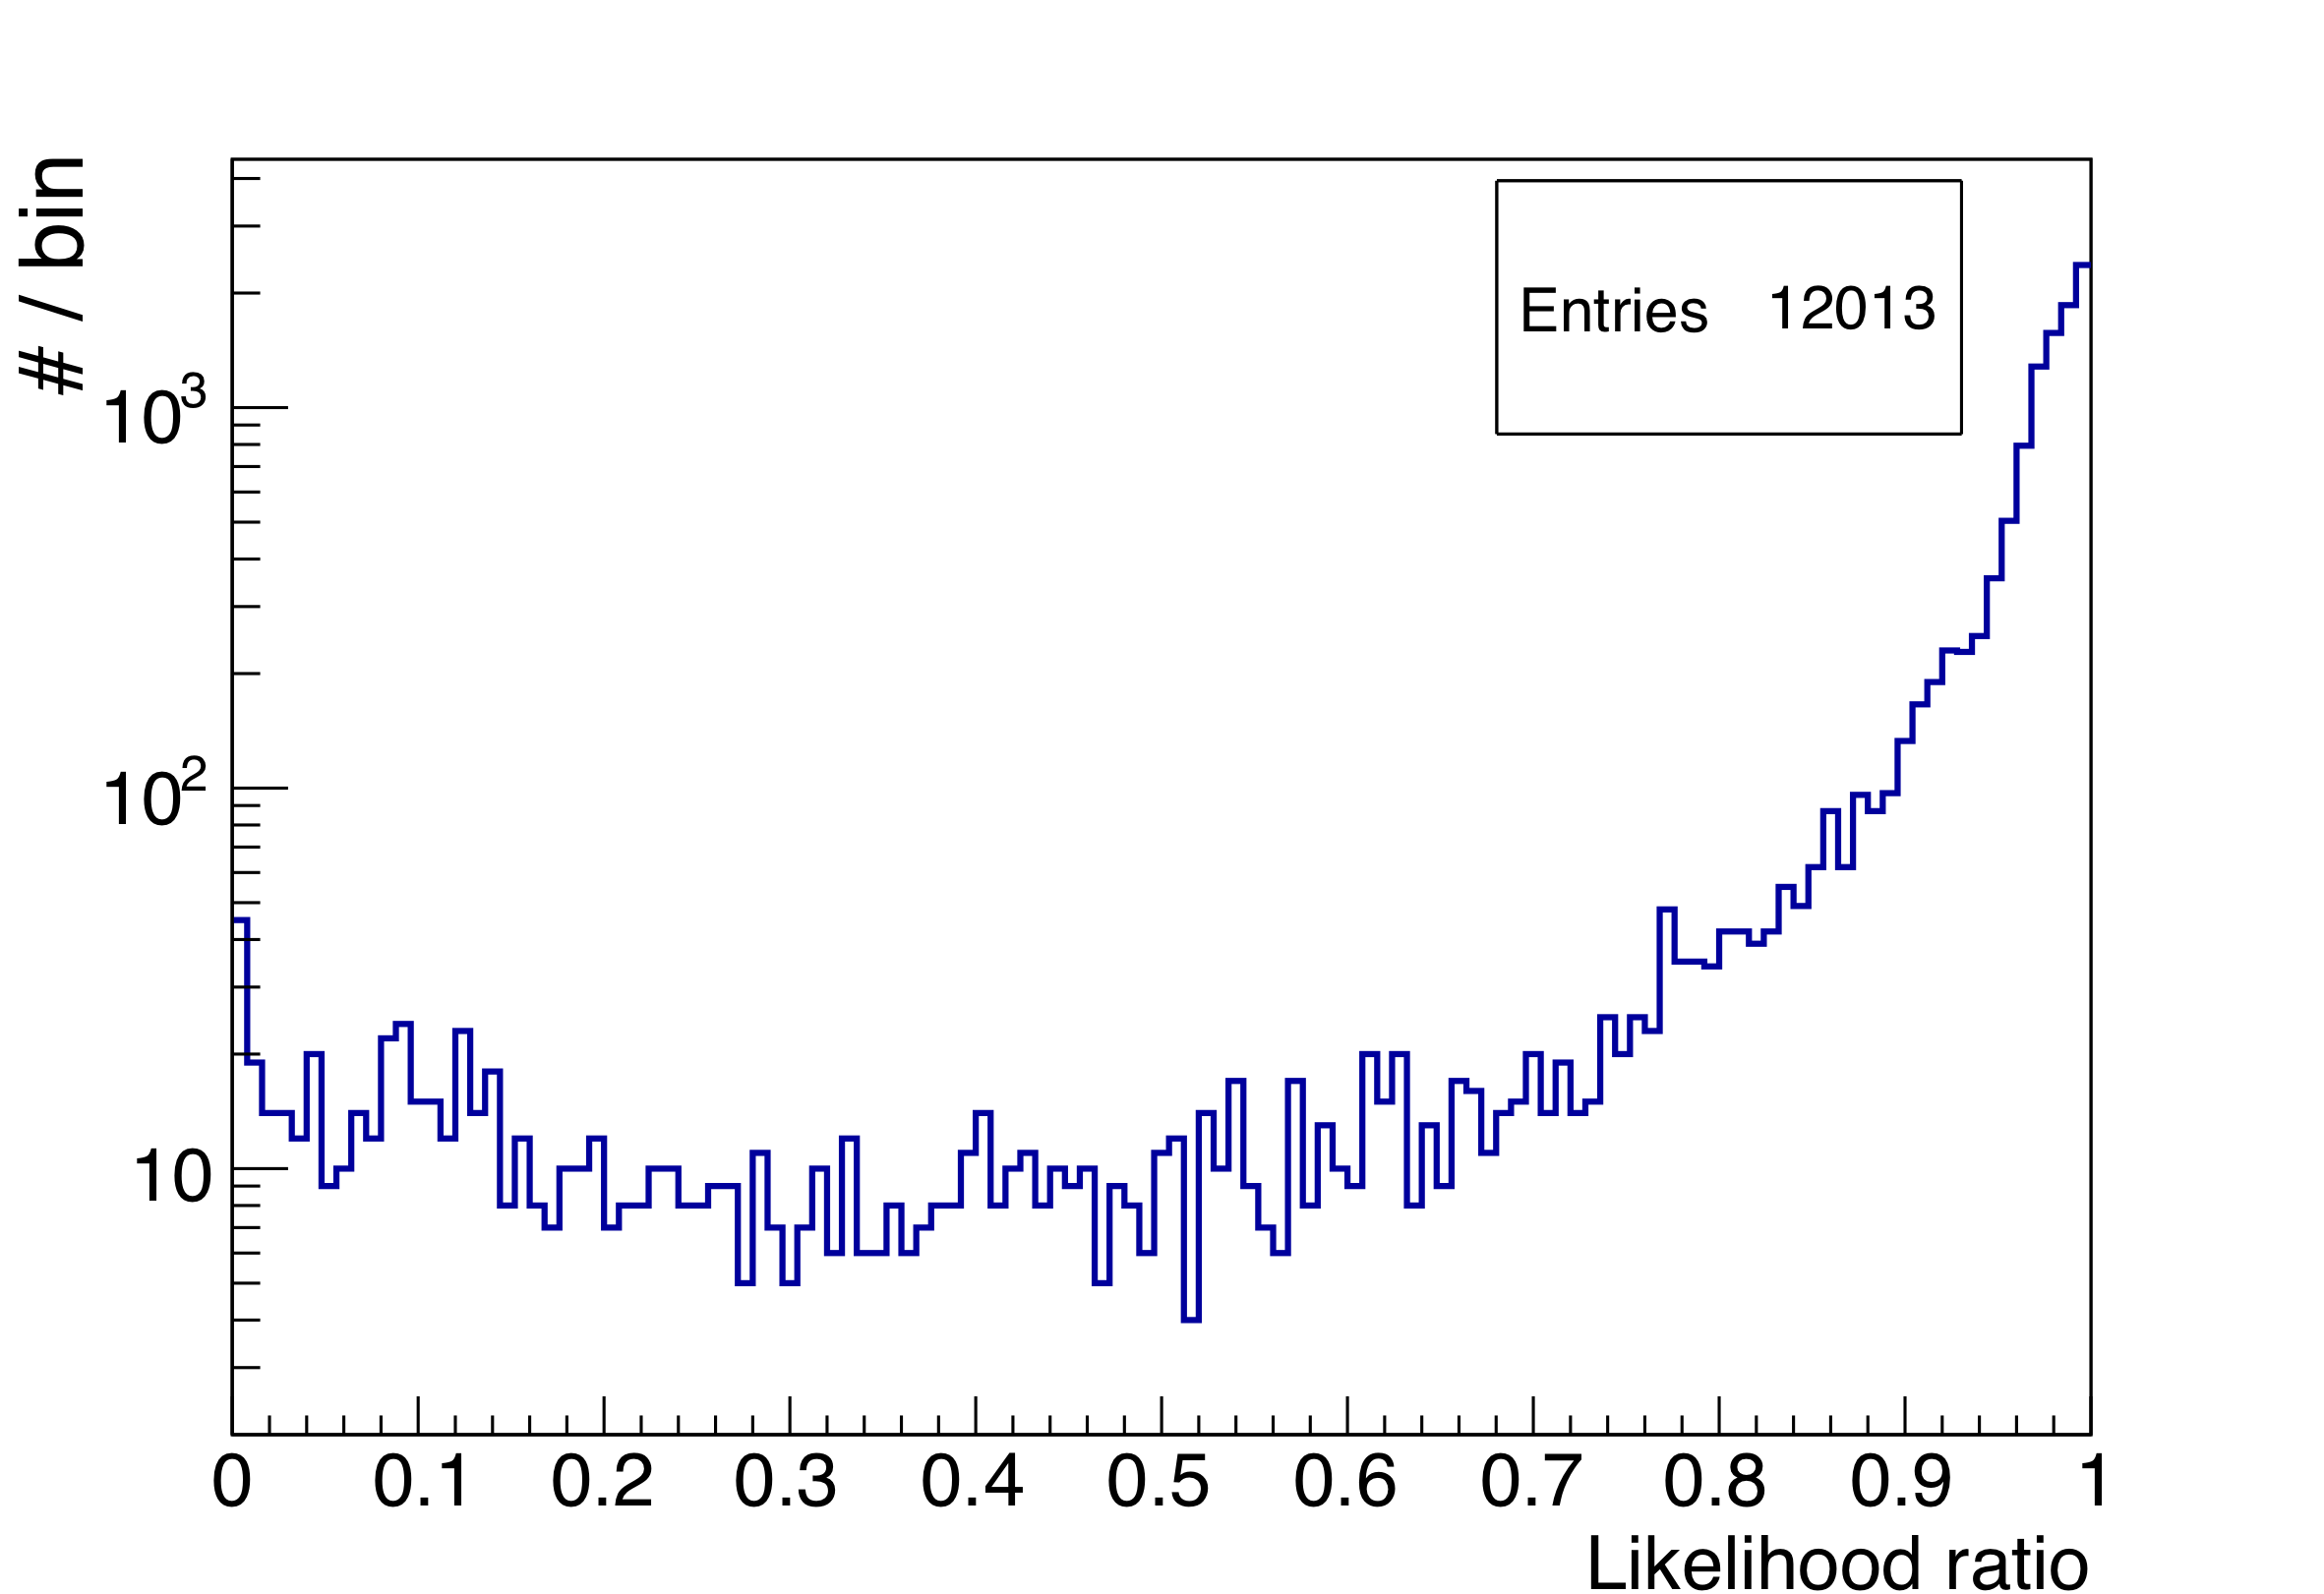
\includegraphics[width=\textwidth]{Figures/scheuch/LikelihoodNonGhost.png}
\caption{Likelihood ratio for an MIP like entry in the calorimeter system for real muons}
\label{LikelihoodReal}
\end{minipage}
\end{figure}
\begin{figure}
\begin{minipage}[t]{0.95\textwidth}
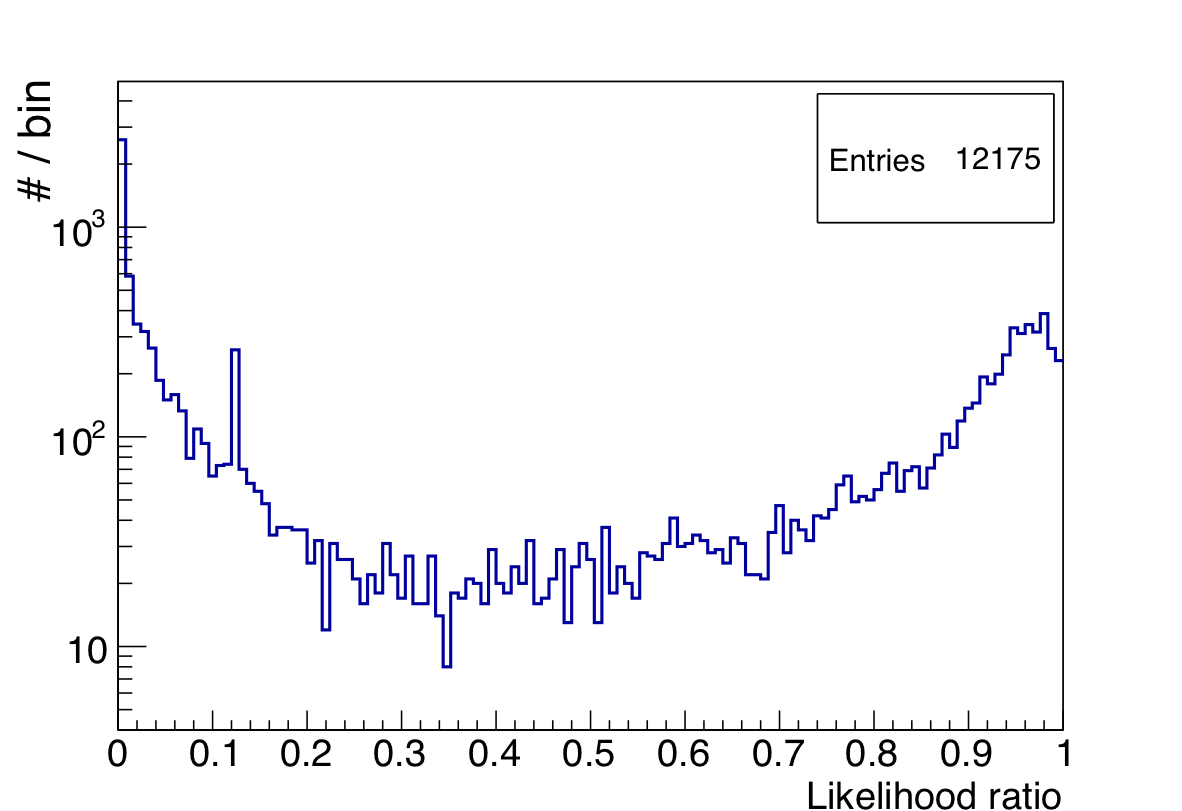
\includegraphics[width=\textwidth]{Figures/scheuch/LikelihoodGhost.png}
\caption{Likelihood ratio for an MIP like entry in the calorimeter system for ghosts}
\label{LikelihoodGhost}
\end{minipage}
\end{figure}
For identified muons the likelihood ratio peaks at 1. This is consistent with the fact that real muons should deposit energy within the calorimeter system.\\
The likelihood ratio for ghosts peaks at 0, has a miminum at 0.4, and rises again up to 1 without reaching a maximum at 1. The ghosts should not deposit energy in the calorimeter system. For some of the ghosts this seems to be the case. For the other ghosts the likelihood might be tending to 1 because energy is deopsited in the calorimeter system by other particles or due to some noise. This can also explain why the likelihood ratio drops at the 1st bin for ghosts.\\
In a next step, the energy information in the HO system for an HO tower has to be investigated to obtain whether HO can serve as muon veto and trigger. This has to be redone also for HL-LHC conditions. Here, one has to check whether the granularity of HO is sufficient to deal with the additional pile up and boosted events.
\subsection{BTI Ghosts}
\subsubsection{Ghost definition}
If only one muon passes a muon station and two BTI HQTR are created in this station it is called BTI ghost. (For the description of the BTI system see chapter \ref{DTSystem}.)
\subsubsection{Investigation of the BTI Trigger}
To see whether the BTI triggers experience ghost phenomena, a muon gun study was performed. Events without pileup were created. Every event contains one muon that is passing directly through one of the 12 sectors. This muon hits all four muon chambers. A second muon was shot through a sector next to the sector of the first muon. The number of BTI triggers in the first station was counted.\\
The efficiency is defined as
\begin{equation}
E=\frac{\sum_{i = 1}^\infty N_{\mathrm{BTI}_i}}{\sum_{i = 0}^\infty N_{\mathrm{BTI}_i}}
\end{equation}
with $N_{\mathrm{BIT}_i}$ the number of events with $i$ BTI triggers.\\
An effiency of about 80\% is reached for one station only (see Fig. \ref{BTIEfficiency}).
\begin{figure}
\begin{minipage}[t]{0.95\textwidth}
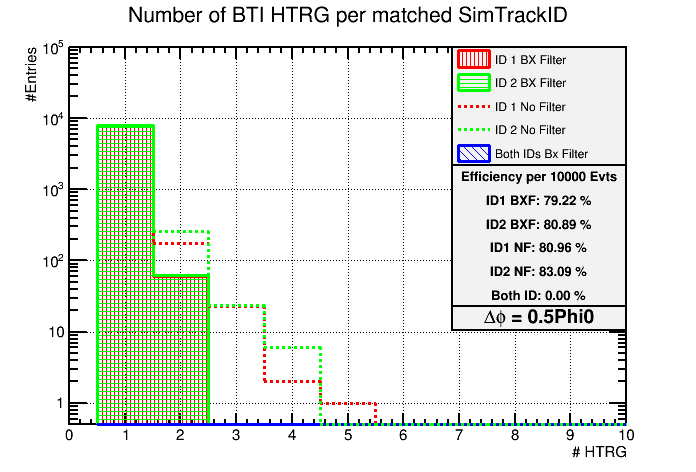
\includegraphics[width=\textwidth]{Figures/scheuch/SectorGunPt100dPhi0_5Phi0_h1dFilteredBtiHitsPerEvtSL1.png}
\caption{Number of BTI trigger in station one for one passing muon and BTI trigger efficiency}
\label{BTIEfficiency}
\end{minipage}
\end{figure}
The number of events with BTI ghosts is defined as
\begin{equation}
N_{\mathrm{Ghost\ Event}} = \sum_{i = 2}^\infty N_{\mathrm{BTI}_{i\cdot}}
\end{equation}
This number can be up to 5 if no filter on the bunchcrossing ID is used. The filter on the bunchcrossing ID can reduce this number of BTI ghosts significantly. Using the filter on the bunchcrossing ID the ghost rate at BTI level is reduced to about 1\%.\\
Unfortunately, an adjustment oder modification of the BTI system is not possible for the planned upgrade phases since it would need direct access to every muon station. Therefore, the number of BTI trigger can not be reduced by an HO like system.